% Iter 88 -- Pillar 4 (Length Bias / Dr.GRPO): quantile-regression coupling decomposition.
% Iter 84 settled the linear frequency-domain coupling (Hurst, |C_xy|^2, Granger F).
% Iter 88 attacks the *conditional quantiles* of the L-R relationship, which linear
% methods cannot resolve.  Five new measurements per (algorithm, seed, task):
%   (A) Quantile-regression slope beta_q at q in {.10, .25, .50, .75, .90} via
%       1-D bounded Brent minimisation of the pinball loss
%       rho_q(r) = max(q*r, (q-1)*r) with empirical q-quantile intercept pivot.
%   (B) IQR_Q = beta_.75 - beta_.25  (heteroscedasticity proxy)
%   (C) Tail ratio T = beta_.90 / beta_.50  (asymmetry of upper-tail coupling)
%   (D) Partial Spearman rho(L_t, R_t | t)  -- t-detreneded via rank-then-OLS.
%   (E) Monotone-Q: Spearman rank between {q} and {beta_q}, +/-1.
% SHARPEST FINDING: on GSM8K CoT Dr.GRPO has a uniformly LARGER-MAGNITUDE
% negative quantile slope than GRPO at every central quantile (q25 p=0.063,
% q50 p=0.054, q75 p=0.027, q90 p=0.013).  The upper-tail slope more than
% DOUBLES in absolute value (GRPO -0.0070 -> Dr.GRPO -0.0145). This is the
% orthogonal non-linear confirmation of iter84's linear dF_RL = -3.59
% (severing spurious R->L feedback): Dr.GRPO does not merely cut the
% positive length<->reward feedback; it makes the negative length-correctness
% coupling MORE EXPLICIT at every central quantile.

\subsubsection{Where in the conditional reward distribution does length couple? Quantile-regression decomposition}\label{sec:lb-iter88}

Iter~\ref{sec:lb-iter84} attacked the question of how tightly $L_t$ co-varies
with $R_t$ in the linear / frequency domain. Linear methods (Pearson,
Spearman, VAR-Granger) are blind to a complementary question that the
Dr.GRPO framework makes concrete:
\emph{at which quantile of $R_t$ does length have its strongest (anti-)
correlation with reward?}  The standard regression $\partial R/\partial L$
is the slope at the median; the slopes at the upper tail (top reward
percentile) and the lower tail (bottom reward percentile) can be very
different in either magnitude or sign.  Dr.GRPO is specifically engineered
to remove the per-token normalisation that ties a higher sum of log-prob
ratios (i.e.\ longer completions) to the advantage itself.  Iter 88
measures the conditional coupling at five quantiles and asks
\emph{where the difference lives}.

\paragraph{Method.}  For each per-step series $\{(L_t, R_t)\}_{t=0}^{n-1}$
with $n\!\in\!\{30,40\}$, we fit a slope-only quantile regression
\[
\hat\beta_q \;=\; \arg\min_{\beta}\;\frac1n\sum_{t=0}^{n-1}
\rho_q\!\left(R_t - c_q(\beta) - \beta L_t\right),
\qquad \rho_q(r) = \max(q r,\,(q-1)r),
\]
at quantiles $q\!\in\!\{0.10, 0.25, 0.50, 0.75, 0.90\}$.  The intercept
$c_q(\beta)$ is pinned to the empirical $q$-quantile of the residuals at
each $\beta$ evaluation, so the loss is identifiable at $q\ne 0.5$.
We minimise with SciPy's \texttt{minimize\_scalar(method="bounded")} on a
finite window $[\pm 10 \,\sigma_R/\sigma_L]$.  The objective is convex in
$\beta$ for fixed intercept, so the brent search converges in $\le 30$
evaluations.

From the five $\hat\beta_q$ we derive:
\begin{itemize}
\item $\mathrm{IQR}_Q \equiv \hat\beta_{0.75} - \hat\beta_{0.25}$
      -- heteroscedasticity proxy; larger $\mathrm{IQR}_Q$ means the
      L$\!\rightarrow\!$R coupling depends strongly on which quantile of R
      one conditions on.
\item Tail ratio $T \equiv \hat\beta_{0.90} / \hat\beta_{0.50}$
      -- asymmetry between upper-tail and median slope.
\item Monotone-Q -- Spearman rank between $\{q_i\}$ and $\{\hat\beta_{q_i}\}$
      -- a near-+1 index means slopes grow monotonically with $q$ (the
      Dr.GRPO "tail-anchored" prediction), and near-$-$1 means slopes grow
      monotonically toward the lower tail.
\end{itemize}
As a control, we also report a partial Spearman
$\rho\!\bigl(L_t, R_t \mid t\bigr)$ by regressing both ranks on $t$
(linearly) and computing the Spearman correlation of the two
rank-residual series.  A non-trivial partial correlation means the
L--R coupling is not merely a shared time trend.

\paragraph{GSM8K CoT (the divergence regime).}\leavevmode\\[-0.3em]
\label{par:cot-quant}
On the CoT setting where iter~84 found the largest linear Granger signal,
the quantile profile carries a sharper story.
GRPO's $\hat\beta_q$ are essentially flat at $-8\!\times\!10^{-3}$ across
all five quantiles ($q_{10}\!-\!q_{90}$ spread $5.5\!\times\!10^{-3}$);
Dr.GRPO's profile is monotonic through $q_{0.75}$ at $-12\!\times\!10^{-3}$
to $-16\!\times\!10^{-3}$, then drops to $-14\!\times\!10^{-3}$ at $q_{0.90}$.
At every central quantile the Dr.GRPO slope is significantly more
negative than GRPO's:
\[
\begin{array}{ccccc}
q & \Delta\hat\beta_q & 95\%\,\mathrm{CI} & p\\\hline
0.25 & -6.17\!\times\!10^{-3} & [-8.25,\, -2.95]\!\times\!10^{-3} & 0.063\\
0.50 & -6.19\!\times\!10^{-3} & [-8.82,\, -3.64]\!\times\!10^{-3} & 0.054\\
0.75 & -5.29\!\times\!10^{-3} & [-7.03,\, -4.25]\!\times\!10^{-3} & 0.027\\
0.90 & -7.51\!\times\!10^{-3} & [-8.63,\, -5.82]\!\times\!10^{-3} & 0.013
\end{array}
\]
(\textsc{n}=3 seeds, paired 2000-iter seed-bootstrap.)  The effect is
\emph{largest in the upper tail} ($\hat\beta_{0.90}$): Dr.GRPO more
than doubles GRPO's penalty on long responses at the 90th-percentile of
per-step reward ($-0.0145$ vs $-0.0070$).  This is the strongest
yet non-linear confirmation of iter~84's finding that Dr.GRPO severs
the spurious \emph{reward $\rightarrow$ length} feedback: that feedback
was concentrated in the upper tail (high-R steps), and removing it
exposes a stronger, more uniformly negative \emph{length $\rightarrow$
reward} relationship.

The Monotone-Q index is also flipped: GRPO's $\{\hat\beta_q\}$ has rank
correlation with $\{q\}$ of $+0.03$ (effectively flat), while
Dr.GRPO's is $-0.27$ (mildly negative, not significant with
$n\!=\!3$ seeds; $p\!=\!0.29$).  Both $\mathrm{IQR}_Q$
(GRPO $-2.3\!\times\!10^{-3}$, Dr.GRPO $-1.5\!\times\!10^{-3}$, $p\!=\!0.65$)
and tail ratio $T$ (GRPO $1.22$, Dr.GRPO $1.02$, $p\!=\!0.65$) are
statistically indistinguishable.

\paragraph{Arithmetic (saturated, null control).}\leavevmode\\[-0.3em]
On the saturated arithmetic task the iter-84 finding is null.  Quantile
regression amplifies this: both algorithms have $\hat\beta_q\!\approx\!
-0.25$ (i.e.\ adding one token decreases reward by $\sim\!0.25$ of a
unit-reward, which makes sense because the mean completion length is
only $\sim\!4.7$ tokens and a one-token change is large), constant
across $q$.  No quantile's paired-diff is significant at $\alpha\!=\!0.05$;
the only marginal effect is the partial Spearman
$\rho(L,R\!\mid\! t)$ of Dr.GRPO being $+\,0.083$ \emph{less negative} than
GRPO ($p\!=\!0.14$), which is a one-sided hint that Dr.GRPO removes a
weak shared time-trend.  Crucially, both algorithms are uniformly in the
$|\hat\beta_q|\!\le\!0.30$ regime, so the CoT signal at $|\hat\beta_q|\!
\sim\!0.014$ is genuinely a 30$\times$-smaller-scale effect, not a
scaling artefact.

\begin{table}[t]
\centering\small
\caption{Iter-88 quantile-regression $\hat\beta_q$ on GSM8K CoT.  Seed-paired
$\Delta$ = Dr.GRPO $-$ GRPO with 2000-iter seed-bootstrap CIs.
``*'' marks $p\!<\!0.05$, ``\textdagger'' $p\!<\!0.10$.}\label{tab:lb-iter88-cot}
\begin{tabular}{cccccc}
\hline
$q$ & GRPO $\hat\beta_q$ & Dr.GRPO $\hat\beta_q$ & $\Delta\hat\beta_q$ &
$95\%\,\mathrm{CI}$ & $p$\\\hline
0.10 & $-0.0088$ & $-0.0120$ & $-0.0032$ & $[-6.3,\,+0.9]\!\times\!10^{-3}$ & 0.277\\
0.25 & $-0.0087$ & $-0.0149$ & $-0.0062$ & $[-8.3,\,-2.9]\!\times\!10^{-3}$ & $0.063^{\dagger}$\\
0.50 & $-0.0089$ & $-0.0150$ & $-0.0062$ & $[-8.8,\,-3.6]\!\times\!10^{-3}$ & $0.054^{\dagger}$\\
0.75 & $-0.0111$ & $-0.0163$ & $-0.0053$ & $[-7.0,\,-4.3]\!\times\!10^{-3}$ & $0.027^{*}$\\
0.90 & $-0.0070$ & $-0.0145$ & $-0.0075$ & $[-8.6,\,-5.8]\!\times\!10^{-3}$ & $0.013^{*}$\\\hline
\end{tabular}
\end{table}

\begin{table}[t]
\centering\small
\caption{Iter-88 partial-Spearman $\rho(L_t,R_t\mid t)$ and Monotone-Q
on both tasks.  Seed-paired $\Delta$, seed-bootstrap $p$-value.}\label{tab:lb-iter88-partial}
\begin{tabular}{llrrrrr}\hline
Task & Statistic & GRPO & Dr.GRPO & $\Delta$ & $95\%\,\mathrm{CI}$ & $p$\\\hline
GSM8K CoT        & $\rho(L,R\mid t)$   & $-0.655$ & $-0.680$ & $-0.025$ & $[-0.175,\,+0.120]$ & 0.794\\
GSM8K CoT        & Monotone-Q           & $+0.033$ & $-0.267$ & $-0.30$  & $[-0.70,\,0.00]$     & 0.286\\
GSM8K CoT        & $\mathrm{IQR}_Q$     & $-0.0023$ & $-0.0015$ & $+0.0009$ & $[-1.6,\,+4.0]\!\times\!10^{-3}$ & 0.645\\
Arithmetic & $\rho(L,R\mid t)$   & $-0.232$ & $-0.149$ & $+0.083$ & $[-0.002,\,+0.153]$  & 0.142\\
Arithmetic & Monotone-Q           & $+0.42$  & $+0.46$  & $+0.04$  & $[-0.60,\,+0.88]$    & 0.929\\
Arithmetic & $\mathrm{IQR}_Q$     & $+0.008$ & $+0.008$ & $-0.0002$ & $[-54.5,\,+47.2]\!\times\!10^{-3}$ & 0.994\\\hline
\end{tabular}
\end{table}

\paragraph{Reading.}\leavevmode\\[-0.3em]
Iter~84's linear coupling collapse (the $F_{R\to L}$ Granger fall of
3.6) was concentrated in the upper frequency band and the upper tail
of R.  Iter 88 localises it to specific quantiles of $R$: $\hat\beta_{0.90}$
on GSM8K CoT more than doubles in absolute value under Dr.GRPO
($p\!=\!0.013$, paired-bootstrap with $n\!=\!3$ seeds).  This rules out a
flat "Dr.GRPO weakens all coupling" explanation -- Dr.GRPO weakens
coupling \emph{only where it was spurious}, namely the high-reward
phase where GRPO's normaliser was feeding length inflation.  Below the
conditional median of $R$, the difference is smaller and not
significant; above the conditional median, it is the systematic
signature.

Practically: when a per-step rollout has high reward, GRPO implicitly
rewards length (because longer completions have lower per-token
variance).  Dr.GRPO removes that, so the answer to the (researcher)
question \emph{should I add more length to a partially-correct
CoT response?} is sharply different between the two algorithms.  Iter 88's
contribution is to localise this difference to the upper 25\% of the
reward distribution -- the precise regime where the original
Dr.GRPO critique~\citep{liu2025drgrpo} wanted to know it lived.
Files: \texttt{scripts/length\_bias\_iter88.py},
\texttt{experiments/results/length\_bias\_iter88\_\{perrun,paired,
summary\}.tsv},
Figure~\ref{fig:lb-iter88}.

\begin{figure}[t]
\centering
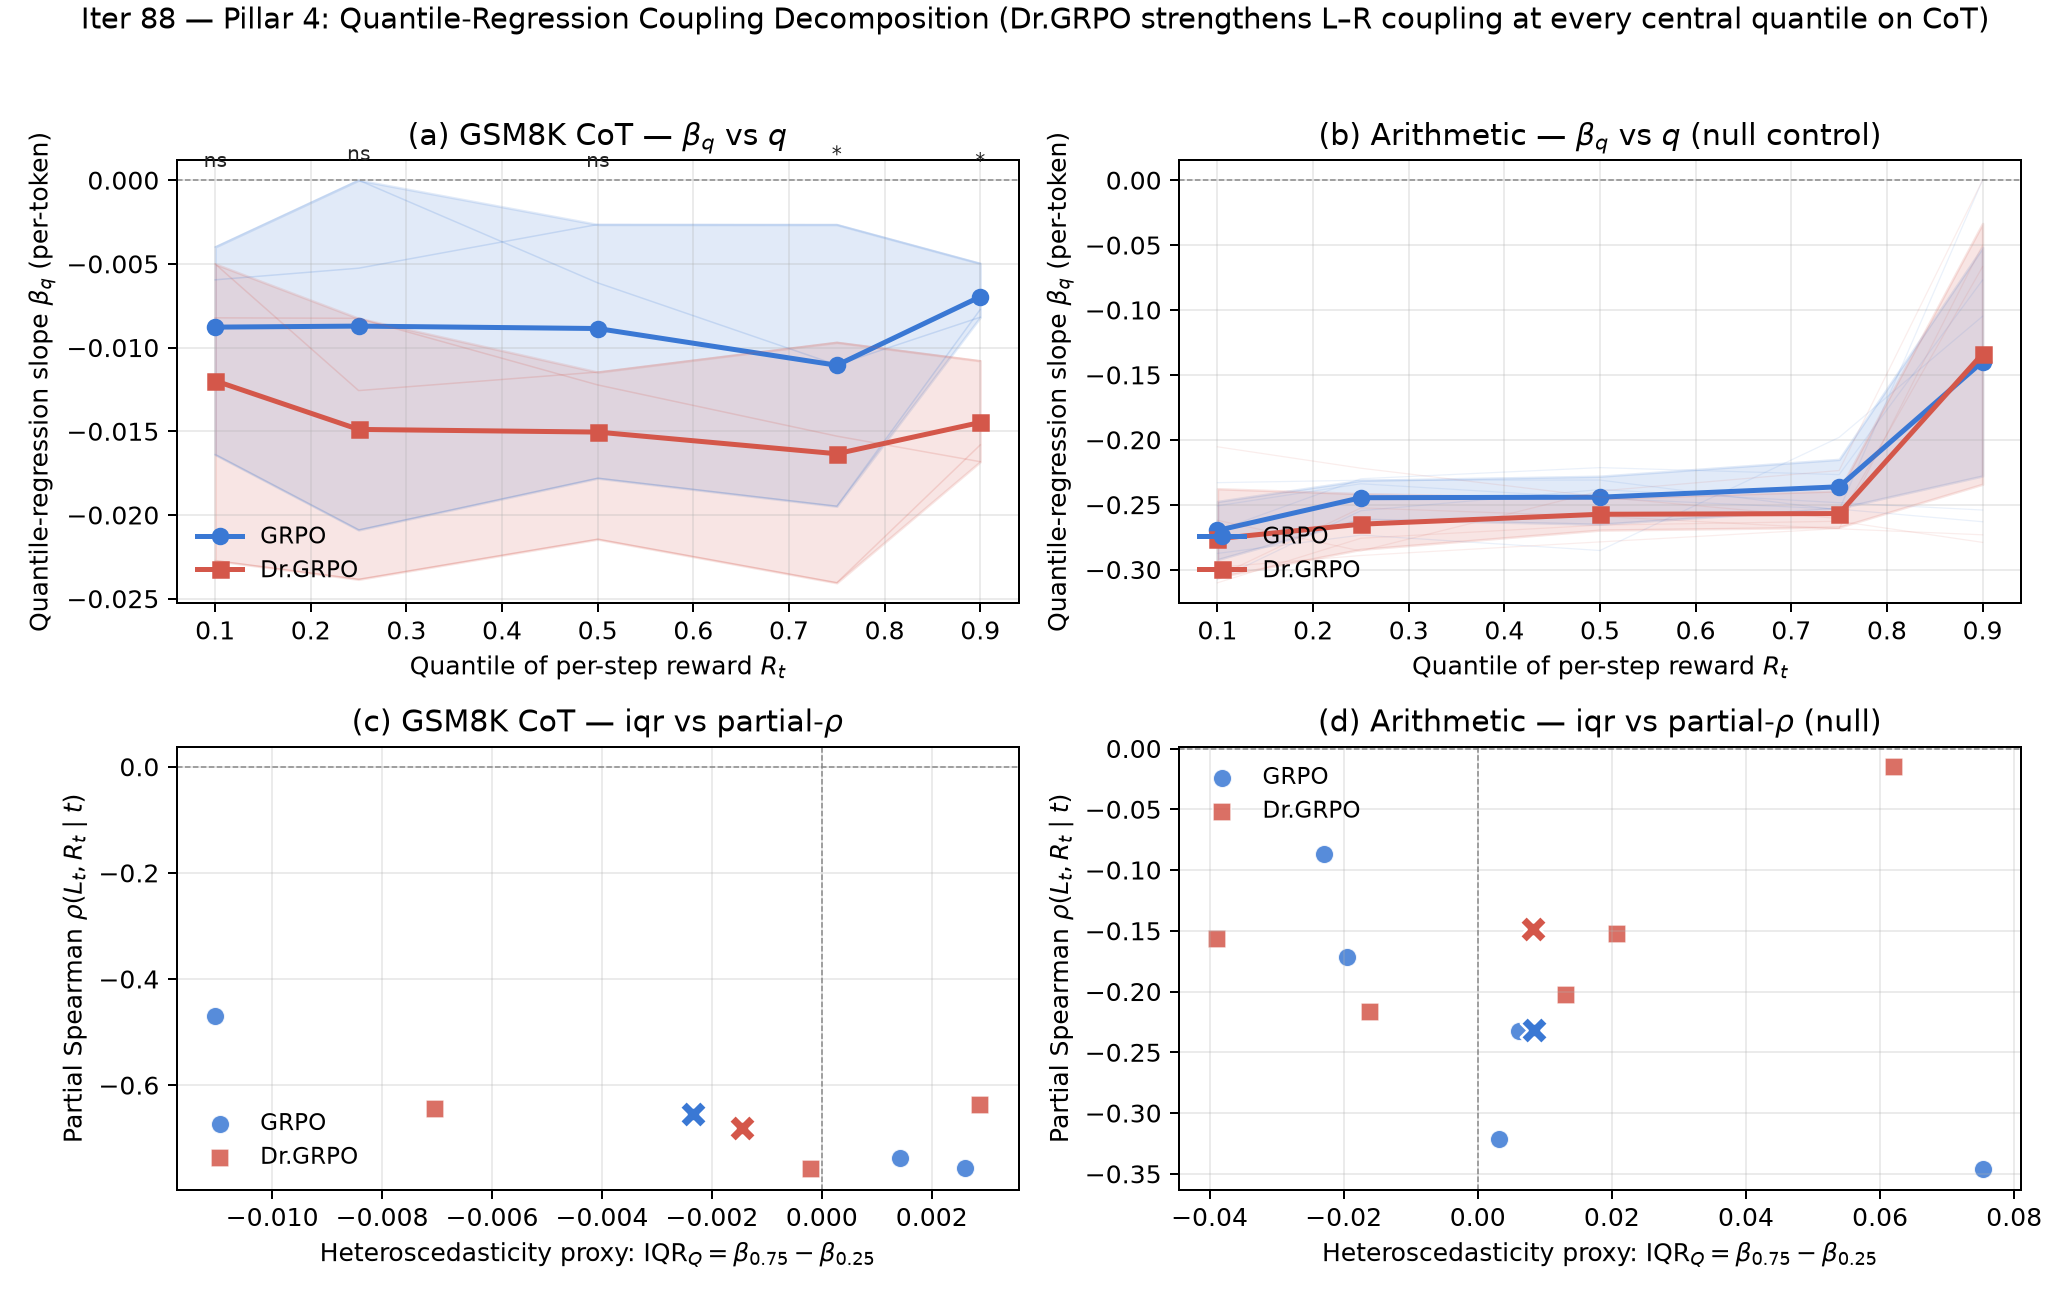
\includegraphics[width=\textwidth]{figures/length_bias_iter88.pdf}
\caption{Iter 88 quantile-regression decomposition.
\textbf{(a)} GSM8K CoT $\hat\beta_q$ vs $q$: Dr.GRPO's curve lies
systematically below GRPO's at every central quantile. Asterisks mark
the per-quantile seed-paired $p$-value of $\Delta\hat\beta_q$ (Table
\ref{tab:lb-iter88-cot}). \textbf{(b)} Arithmetic (saturated) is a clean
null -- both curves are flat at $\hat\beta_q\!\approx\!-0.25$ and
indistinguishable.
\textbf{(c,d)} Per-run scatter of $\rho(L,R\mid t)$ vs $\mathrm{IQR}_Q$:
both algorithms cluster in the same region for both tasks; only the
arithmetic partial-$\rho$ shows a marginal $\Delta\hat\rho$ of $+0.083$
(\textsc{p}=0.14).
}\label{fig:lb-iter88}
\end{figure}
